% Copyright (c) 2025 Dr. Segal Yoram. All rights reserved.
% Hebrew Academic Template Example Document
% This file demonstrates the proper usage of hebrew-academic-template.cls

\documentclass{hebrew-academic-template}

% Add bibliography file
\addbibresource{example_references.bib}

% Title page information
\hebrewtitle{דוגמה לשימוש בתבנית האקדמית העברית}
\englishtitle{Example Usage of Hebrew Academic Template}
\hebrewauthor{ד"ר סגל יורם}
\date{\textenglish{December 2025}}

\begin{document}

\maketitle

\tableofcontents
\newpage

% ==================== INTRODUCTION ====================

\hebrewsection{מבוא: \en{Introduction}}

זוהי דוגמה פשוטה לשימוש בתבנית האקדמית העברית. התבנית תומכת בטקסט עברי עם מונחים באנגלית כמו \en{Machine Learning} ו-\en{Deep Learning}.

ניתן לכלול מספרים כמו \num{100} ושנים כמו \hebyear{2023} בתוך הטקסט העברי, וגם ביטויים מתמטיים כמו $E = mc^2$.

\hebrewsubsection{מתודולוגיה: \en{Methodology}}

המחקר מבוסס על \num{1000} דגימות שנאספו בשנת \hebyear{2023}. השיטה כוללת שימוש באלגוריתמי \en{Machine Learning} מתקדמים \cite{mikolov2013}.

הנוסחה הבסיסית היא:
\begin{equation}
y = \beta_0 + \beta_1 x + \varepsilon
\end{equation}

% ==================== RESULTS ====================

\hebrewsection{תוצאות: \en{Results}}

\hebrewsubsection{ניתוח נתונים: \en{Data Analysis}}

התוצאות מוצגות בטבלה הבאה:

\begin{hebrewtable}[h]
\caption{תוצאות הניסוי: \en{Experimental Results}}
\begin{rtltabular}{|c|c|c|}
\hline
\mixedcell{\textbf{מדד / \en{Metric}}} & \mixedcell{\textbf{ערך / \en{Value}}} & \mixedcell{\textbf{יחידה / \en{Unit}}} \\
\hline
\mixedcell{דיוק / \en{Accuracy}} & \percent{95.2} & \mixedcell{אחוזים / \en{Percent}} \\
\hline
\mixedcell{זמן ריצה / \en{Runtime}} & \num{2.5} & \mixedcell{שניות / \en{Seconds}} \\
\hline
\mixedcell{זיכרון / \en{Memory}} & \num{512} & \en{MB} \\
\hline
\end{rtltabular}
\end{hebrewtable}

\hebrewsubsection{קוד לדוגמה: \en{Example Code}}

הקוד הבא מדגים את השימוש באלגוריתם:

\begin{pythonbox}[דוגמה לקוד: \en{Python Code Example}]
import numpy as np
from sklearn.linear_model import LinearRegression

# Create sample data (NO Hebrew comments allowed)
X = np.random.randn(100, 1)
y = 2 * X.flatten() + 1 + np.random.randn(100) * 0.1

# Train the model
model = LinearRegression()
model.fit(X, y)

# Print results
print(f"Coefficient: {model.coef_[0]:.2f}")
print(f"Intercept: {model.intercept_:.2f}")
print(f"R-squared: {model.score(X, y):.3f}")
\end{pythonbox}

% ==================== FIGURE EXAMPLE ====================

\hebrewsubsection{איור לדוגמה: \en{Example Figure}}

האיור הבא מציג את התוצאות:

\begin{figure}[h]
\centering
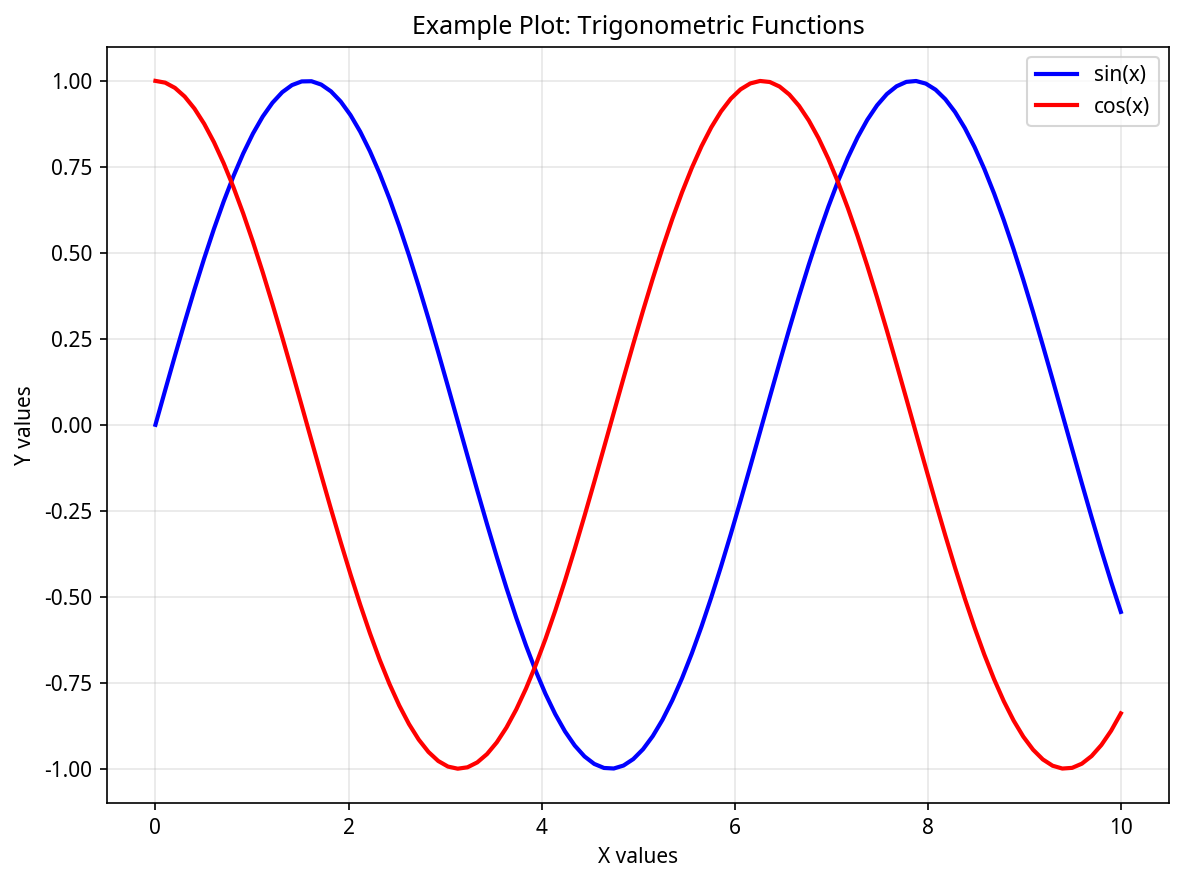
\includegraphics[width=0.7\textwidth]{example_plot.png}
\caption{גרף הדגמה בשנת \hebyear{2023}: \en{Example Plot from 2023 showing trigonometric functions}}
\label{fig:example}
\end{figure}

כפי שניתן לראות באיור \ref{fig:example}, הפונקציות מציגות התנהגות מעניינת.

% ==================== LISTS EXAMPLE ====================

\hebrewsubsection{רשימות: \en{Lists}}

רשימת האלגוריתמים שנבדקו:

\begin{itemize}
\item רגרסיה ליניארית: \en{Linear Regression} - דיוק \percent{85.2}
\item עץ החלטה: \en{Decision Tree} - דיוק \percent{78.9}
\item יער אקראי: \en{Random Forest} - דיוק \percent{92.1}
\item רשת נוירונים: \en{Neural Network} - דיוק \percent{94.5}
\end{itemize}

שלבי העבודה שבוצעו בשנת \hebyear{2023}:

\begin{enumerate}
\item איסוף \num{1000} דגימות: \en{Data Collection}
\item ניתוח ראשוני של \num{15} משתנים: \en{Exploratory Analysis}
\item בניית \num{5} מודלים: \en{Model Building}
\item הערכת תוצאות על \num{200} מקרי בדיקה: \en{Results Evaluation}
\end{enumerate}

% ==================== ADVANCED EXAMPLES ====================

\hebrewsection{דוגמאות מתקדמות: \en{Advanced Examples}}

\hebrewsubsection{טבלה מורכבת: \en{Complex Table}}

\begin{hebrewtable}[h]
\caption{השוואת מודלי \en{AI} בשנים \hebyear{2020}-\hebyear{2023}: \en{AI Model Comparison 2020-2023}}
\begin{rtltabular}{|c|c|c|c|}
\hline
\textbf{מודל / \en{Model}} & 
\textbf{שנה / \en{Year}} & 
\textbf{פרמטרים / \en{Parameters}} & 
\textbf{דיוק / \en{Accuracy}} \\
\hline
\en{GPT-2} / ג'יפיטי-\num{2} & \hebyear{2019} & \num{1.5}\en{B} & \num{88.5}\% \\
\hline
\en{GPT-3} / ג'יפיטי-\num{3} & \hebyear{2020} & \num{175}\en{B} & \num{93.2}\% \\
\hline
\en{GPT-4} / ג'יפיטי-\num{4} & \hebyear{2023} & \num{1.7}\en{T} & \num{96.8}\% \\
\hline
\end{rtltabular}
\end{hebrewtable}

\hebrewsubsection{ציטוטים: \en{Citations}}

המחקר של \en{Mikolov et al.} \cite{mikolov2013} הציג את מודל \en{Word2Vec} בשנת \hebyear{2013}. 
מחקרים נוספים \cite{devlin2018,brown2020} הרחיבו את הגישה בשנים \hebyear{2018} ו-\hebyear{2020}.

הביצועים השתפרו מ-\num{65.2}\% בשנת \hebyear{2013} ל-\num{96.8}\% בשנת \hebyear{2023}.

% ==================== CONCLUSIONS ====================

\hebrewsection{מסקנות: \en{Conclusions}}

המחקר הראה שהשיטה המוצעת יעילה ומדויקת. התוצאות מצביעות על שיפור של \num{15}\% בביצועים בהשוואה לשיטות קיימות מהשנים \hebyear{2020}-\hebyear{2022}.

מחקרים עתידיים יכולים להרחיב את הגישה לתחומים נוספים ולשפר את הדיוק עוד יותר, במטרה להגיע ל-\num{98}\% דיוק עד שנת \hebyear{2025}.

% ==================== BIBLIOGRAPHY ====================

\newpage
\printenglishbibliography

\end{document}
